\section{Grundlagen}
%*Im Folgenden Kapitel werden die Grundlagen erklärt die Notwenig sind um die 
% Aufgabe zu verstehen. Es werden nur auf die Eigenschaften eingegangen die Nötig sind um die fortlaufende
%Arbeit zu verstehen. "Irgendwie so etwas in die richtung "
\subsection{Qubits} 
"`Der Anfang enthält also beides, Sein und
Nichts; ist die Einheit von Sein und Nichts,
– oder ist Nichtsein, das zugleich Sein, und
Sein, das zugleich Nichtsein ist."'
- Georg Wilhelm Friedrich Hegel

Die Repräsentation und Speicherung von Information ist ein zentraler Aspekt aller Computer, 
unabhängig von der verwendeten Technologie oder Architektur. 
Bei klassischen Computern basiert diese Repräsentation auf dem Binärsystem. 
In der klassischen Repräsentation ist das Bit die kleinste Informationseinheit, 
die eine von zwei mögliche Zustände annehmen kann: 0 oder 1. 
Ein Bit hat zu jedem Zeitpunkt einen klar definierten Zustand. 
Mehrmaliges Auslesen eines Bits führt zu keiner Zustandsänderung, 
sofern keine Operationen zwischen den Auslesungen durchgeführt werden.

Quantencomputer hingegen funktionieren grundlegend anders. 
Sie stützen sich auf die Prinzipien der Quantenmechanik und verwenden anstelle von Bits Quatenbits beziehungsweise Qubits zur Informationsrepräsentation.
Ein einzelnes Qubit stellt die kleinstmögliche Informationseinheit dar über die ein Quantencomputer verfügt.
Um quantenmechanische Zustände von Qubits zu beschreiben wird die Dirac-Notation als mathematische Schreibweise genutzt~\cite{dirac_1939}.

Ein Qubit kann den Zustände 0 oder den Zustand 1 annehmen:
\begin{center}
\(\ket{0}\) oder entsprechend \(\ket{1}\)
\end{center}

Des weiteren kann ein Qubit auch beide der Basiszustände gleichzeitig einnehmen:
\begin{center}
\(\ket{\Psi} = \alpha\ket{0} + \beta\ket{1}\)
\end{center}
Dieses Phänomen ist eine der charakteristischen Eigenschaften von Qubits und wird als \textbf{Superposition} bezeichnet.
Dabei handelt es sich bei den Vorfaktoren \(\alpha\) und \(\beta\) um komplexe Zahlen für die gilt:
\begin{center}
\(\lvert\alpha\rvert^2 + \lvert\beta\rvert^2 = 1\)
\end{center}
Es gibt also unendlich viele Zustände, die ein Qubit in einer Superposition der beiden Basiszustände annehmen kann.

In der klassischen Welt findet man nur schwer eine Analogie zur Superposition. 
Man kann sich dies jedoch in etwa an einer Münze vorstellen~\cite{Hoever2023Münze}:

Ein klassisches Bit kann dabei entweder auf der Kopf- oder auf der Zahl-Seite liegen.
Ein Qubit hingegen ist eine Münze die auf der Kante um die eigene Achse rotiert.
Dabei geben die Vorfaktoren \(\alpha\) und \(\beta\) an,
wie die Münze zu der einen oder zu der anderen Seite tendiert.
Ohne die Münze zu beeinflussen ist es nicht möglich die Tendenz, 
also die Vorfaktoren, zu bestimmen.

Möchte man nun aber doch ein konkretes Ergebnis haben, 
muss man das Qubit lesen, 
beziehungsweise genauer gesagt messen.
Dabei wird die Superposition zerstört und das Qubit kollabiert in einen der beiden Basiszustände.

In der Analogie zu der Münze wird die Rotation der Münze gezielt gestoppt, sodass diese auf eine der beiden Seiten kippt.

Die Wahrscheinlichkeiten dafür werden durch die Vorfaktoren des Qubits bestimmt:
\begin{center}
\(\lvert\alpha\rvert^2\) für \(\ket{0}\), \(\lvert\beta\rvert^2\) für \(\ket{1}\)
\end{center}

Es ist also nicht möglich den Zustand eines Qubit während einer Berechnung nur "`anzuschauen"',
da ansonsten die Superposition zerstört wird und sich somit der Zustand des Qubits verändert.
Aus diesem Grund erfolgt die Messung in der Regel erst am Ende eines Quantenalgorithmus, um das endgültige Ergebnis zu ermitteln.

\subsection{Quantengatter}

\subsection{Qiskit}
\subsection{RSA}
%Funktionsweise
%Schwierigkeit Faktorisierung
%Laufzeit klassischer PC

\subsection{Quanten-Fourier-Transformation}
Die Quanten-Fourier-Transformation bildet einen wesentlichen Bestandteil des implementierten Quantenalgorithmus. 
Im folgen Abschnitt wird die allgemeine Anwendung der Quanten-Fourier-Transformation erklärt.
Darüber hinaus wird die Implementierung des Quantenschaltkreis anhand der Formel der Quanten-Fourier-Transformation hergeleitet.

Im Prinzip handelt es sich bei der Quanten-Fourier-Transformation um eine Transformation,
die Qubits von der Standardbasis (\(\ket{0}\), \(\ket{1}\)),
in die entsprechende Fourierbasis (\(\ket{+}\), \(\ket{-}\)) überführt~\cite{homeister2023quantum215}.
Bei dem Basiswechsel werden die Informationen des vorherigen Standardbasiszustandes in die Phase des neuen Zustandes übertragen~\cite{Ruiz-Perez2017}.
Anschließend können in der Fourierbasis Rechnungen durchgeführt werden die im Grunde durch Manipulationen der Phase realisiert werden.
Mit diesem Ansatz ist es möglich arithmetische Operationen, wie beispielsweise 
die Addition, effizienter zu berechnen~\cite{draper2000addition,Ruiz-Perez2017}.

Unter Verwendung der inversen Quanten-Fourier-Transformation, 
die als Rücktransformation dient, 
ist es möglich wieder zurück in die Standardbasis zu transformieren.
Dies bewirkt, die Extraktion der Information aus der Phase in einen messbaren Zustand. 

Die Quanten-Fourier-Transformation ist für ein \(N\) = \(2^n\) mit \(n\) Qubits
für die Basisvektoren \(\ket{x}, x = 0,...,N-1\) wie folgt definiert~\cite{Hoever2023QC}:
\[QFT_{N}\ket{x}_{n} = \frac{1}{\sqrt{N}}\sum_{y=0}^{N-1}  e^{\frac{2 \pi i x y}{N}}\ket{y}_{n}\]
Anhand dieser Definition kann der Quantenschaltkreis nicht direkt hergeleitet werden.
Stattdessen musst die Formel umgeformt werden.

Die folgende Herleitung stammt aus dem Textbuch \textit{Quantum Computation and Quantum Information} Seite 218~\cite{nielsen_chuang_2010}.
Die Herleitung wird der Übersicht halber um Zwischenschritte ergänzt:

Indem \(y\) in der ersten Formel in die Binärschreibweise übertragen wird, erhält man:
%Reihnfolge der Binärschreibweise einheitlich machen
% 
%\begin{align}
%    % -> & <-    &     ->&<-
%    122 &= 3     &   abc &= foo\\
%      x &= y     &
%      a &= 700   &
%\end{align}
%
%\begin{align}
% foo &= bar \\
%     &= baz \\
%     &= woop
%\end{align}
%
\[ y = \sum_{k=1}^{n}2^{n-k} y_{n-k+1}\]  
\begin{align}
  QFT_{N}\ket{x}_{n} &=
    \frac{1}{\sqrt{N}}
    \sum_{y_n=0}^{1} ...
    \sum_{y_1=0}^{1} e^{\frac{2 \pi i x \sum_{k=1}^{n}2^{n-k} y_{n-k+1}}{N}}
    \ket{y_n ... y_{2}y_{1}}
\end{align}
Mit \(N\) = \(2^n\) kann der Bruch im Exponenten gekürzt werden:
\[QFT_{N}\ket{x}_{n} = \frac{1}{\sqrt{N}}\sum_{y_n=0}^{1}...\sum_{y_1=0}^{1}  e^{\frac{2 \pi i x \sum_{k=1}^{n}2^{n-k} y_{n-k+1}}{2^n}}\ket{y_n ... y_{2}y_{1}}\]
\[QFT_{N}\ket{x}_{n} = \frac{1}{\sqrt{N}}\sum_{y_n=0}^{1}...\sum_{y_1=0}^{1}  e^{2 \pi i x \sum_{k=1}^{n}2^{-k} y_{n-k+1}}\ket{y_n ... y_{2}y_{1}}\]
Anschließend kann der Ausdruck \(2^{-k}\) zu \(\frac{1}{2^k}\) umgeformt werden: 
\[QFT_{N}\ket{x}_{n} = \frac{1}{\sqrt{N}}\sum_{y_n=0}^{1}...\sum_{y_1=0}^{1}  e^{\frac{2 \pi i x \sum_{k=1}^{n} y_{n-k+1}}{2^k}}\ket{y_n ... y_{2}y_{1}}\]
Die Summe im Exponenten der Basis \(e\) kann als Produkt umgeschrieben werden.
Anstatt dem Produktzeichen \(\prod\) wird das Tensorprodukt \(\bigotimes\) verwendet, da es sich um Qubits handelt:
\[QFT_{N}\ket{x}_{n} = \frac{1}{\sqrt{N}}\sum_{y_n=0}^{1}...\sum_{y_1=0}^{1} \bigotimes_{k=1}^n{ e^{\frac{2 \pi i x y_k}{2^k}}}\ket{y_{k}}\]
Der Ausdruck kann weiter vereinfacht werden indem das Tensorprodukt vorgezogen wird:
\[QFT_{N}\ket{x}_{n} = \frac{1}{\sqrt{N}}\bigotimes_{k=1}^n [  \sum_{y_k=0}^{1}{ e^{\frac{2 \pi i x y_k}{2^k}}}\ket{y_{k}}]\]
\[QFT_{N}\ket{x}_{n} = \frac{1}{\sqrt{N}}\bigotimes_{k=1}^n [  \ket{0} + { e^{\frac{2 \pi i x}{2^k}}}\ket{1}]\] 
Schreibt man das Tensorprodukt voll aus und notiert \(x\) in Binärschreibweise, erhält man:
\begin{align*}
\frac{1}{\sqrt{N}}\Bigg(
  \ket{0} + { e^{\frac{2 \pi i (2^{n-1}x_n+...+2^1x_2+2^0x_1)}{2^1}}}\ket{1}
  \Bigg)
  &\otimes
  \ket{0} + { e^{\frac{2 \pi i (2^{n-1}x_n+...+2^1x_2+2^0x_1)}{2^2}}}\ket{1} \\
  &\vdotswithin{\otimes} \\
  &\otimes
  \ket{0} + { e^{\frac{2 \pi i (2^{n-1}x_n+...+2^1x_2+2^0x_1)}{2^n}}}\ket{1}
\end{align*}
Die komplexe Exponentialfunktion ergibt für eine natürliche Zahl \(k\): \(e^{2\pi i k} = 1\).
Mit dieser Eigenschaft kann man beispielsweise die Phasenverschiebung des ersten Tensors vereinfachen:
\begin{align*} 
  e^{\frac{2 \pi i (2^{n-1}x_n+ \dotsb +2^1x_2+2^0x_1)}{2^1}}
  &\equiv
  e^{\frac{2 \pi i (2^{n-1}x_n)}{2^1}} \dotsb e^{\frac{2 \pi i (2^1x_2)}{2^1}} e^{\frac{2 \pi i (2^0x_1)}{2^1}} \\
  &\equiv 
  e^{{2 \pi i (2^{n-2}x_n)}} \dotsb e^{{2 \pi i (2^0x_2)}} e^{{2 \pi i (2^{-1}x_1)}}
\end{align*}
Dabei ergibt nur der Term \(e^{{2 \pi i (2^{-1}x_1)}} \neq 1 \)  
und verursacht somit eine relevante Phasenverschiebung.

Abschließend lässt sich das gesamte Tensorprodukt vereinfachen:
\[QFT_{N}\ket{x}_{n} = \frac{1}{\sqrt{N}}(\ket{0} + { e^{\frac{2 \pi i (2^0x_1)}{2^1}}}\ket{1}) \bigotimes
( \ket{0} + { e^{\frac{2 \pi i (2^1x_2+2^0x_1)}{2^2}}}\ket{1})...
( \ket{0} + { e^{\frac{2 \pi i (2^{n-1}x_n+ ... +2^1x_2+2^0x_1)}{2^n}}}\ket{1})\]

Ein einzelner Tensor repräsentiert die Wirkung der Schaltung auf ein einzelnes Qubit.
Somit sind die Phasenverschiebungen erkenntlich die auf ein Qubit wirken.
Ausserdem verdeutlicht die Binärschreibweise dass die angewendete Phasenverschiebung vom Zustand anderer Qubits abhängt.

Für die Implementierung der Quanten-Fourier-Transformation sind nur die Terme relevant
welche eine Phasenverschiebung von \(\neq 1\) bewirken.
Dies kann man mit folgender Formel beschreiben:
\[QFT_{N}\ket{x}_{n} = \frac{1}{\sqrt{N}}\bigotimes_{k=1}^n [  \ket{0} + { e^{\frac{2 \pi i \sum_{b=0}^{k-1}2^b x_{b+1} }{2^k}}}\ket{1}]\] 
Im weiteren wird die Formel verwendet um ein Quantenschaltkreis der Quanten-Fourier-Transformation für drei Qubits zu implementieren:
\[QFT_{8}\ket{x}_{3} = \frac{1}{\sqrt{8}} [ (\ket{0} + { e^{\frac{2 \pi i (2^0x_1)}{2^1}}}\ket{1} ) \bigotimes
( \ket{0} + { e^{\frac{2 \pi i (2^1x_2+2^0x_1)}{2^2}}}\ket{1} ) \bigotimes
( \ket{0} + { e^{\frac{2 \pi i (2^{2}x_3 +2^1x_2+2^0x_1)}{2^3}}}\ket{1} ) ] \]
Man kann die Phasenverschiebung die durch den Zustand eines einzelnen Qubits erzeugt wird verdeutlichen,
indem man die Addition im Exponenten zu einer Multiplikation der gleichen Basen umformt:
\[ = \frac{1}{\sqrt{8}} [ (\ket{0} + { e^{\frac{2 \pi i (2^0x_1)}{2^1}}}\ket{1}) \bigotimes
( \ket{0} + { e^{\frac{2 \pi i (2^1x_2)}{2^2}} e^{\frac{2 \pi i (2^0x_1)}{2^2}} }\ket{1} ) \bigotimes
( \ket{0} + { e^{\frac{2 \pi i (2^{2}x_3)}{2^3}} e^{\frac{2 \pi i (2^1x_2)}{2^3}} e^{\frac{2 \pi i (2^0x_1)}{2^3}}  }\ket{1} ) ] \]
Die Phasenverschiebung wird eindeutiger indem man die Brüche kürzt:
\[ = \frac{1}{\sqrt{8}} [ ( \ket{0} + e^{\pi i x_1}\ket{1} ) \bigotimes
( \ket{0} + { e^{\pi i x_2} e^{ \frac{ \pi i x_1}{2}} }\ket{1} ) \bigotimes
( \ket{0} + { e^{\pi i x_3} e^{\frac{\pi i x_2}{2}} e^{ \frac{ \pi i x_1}{4}} }\ket{1} ) ] \]
In einer abschließenden Umformung lässt sich die \(\frac{1}{\sqrt8}\) aufteilen.
Dadurch erinnern die einzelnen Tensoren,
beziehungsweise Qubits an die Form die bei eine Hadamard-Transformation entsteht:
\[ = \frac{1}{\sqrt{2}}( \ket{0} + e^{\pi i x_1}\ket{1} ) \bigotimes
\frac{1}{\sqrt{2}}( \ket{0} + { e^{\pi i x_2} e^{ \frac{ \pi i x_1}{2}} }\ket{1} ) \bigotimes
\frac{1}{\sqrt{2}}( \ket{0} + { e^{\pi i x_3} e^{\frac{\pi i x_2}{2}} e^{ \frac{ \pi i x_1}{4}} }\ket{1} )  \]
Der Ausdruck \(e^{\pi i x_k}\) ist in jedem der einzelnen Qubits vorhanden.
Des weiteren ist an dem \(x_k\) erkennbar das die angewendete Phasenverschiebung von dem Zustand des Qubits abhängig ist,
auf welches die Verschiebung auch angewendet wird.
Konkret bedeutet dass, das auf jedes Qubit mit dem Zustand \(\ket{x_k} = \ket{1}\) eine Phasenverschiebung von \(e^{\pi i}\) wirkt.
Anhand des ersten Qubits, beziehungsweise Tensor, würde das bedeuten, dass der Zustand bei \(x_1 = 0\)
zu \(\ket{0} + e^{\pi i 0} \ket{1} \equiv \ket{0} + \ket{1}\) wird.
Bei \(x_1 = 1\) würde man \(\ket{0} + e^{\pi i 1} \ket{1}\) erhalten,
was \(\ket{0} - \ket{1}\) entspricht.
Aufgrund des Vorfaktors von \(\frac{1}{\sqrt{2}}\) entsprächen beide Fälle also der Hadamard-Transformation.
Da auch alle anderen Tensoren den Ausdruck \(e^{\pi i x_k}\) und den Vorfaktor \(\frac{1}{\sqrt{2}}\) beinhalten, wirkt auf jedes Qubit ein Hadamard-Gatter.

Die weiteren Tensoren des Tensorproduktes beinhalten zunehmend mehr Ausdrücke die für unterschiedliche Phasenverschiebungen sorgen.
Die Phasenverschiebung von einem einzelnen Ausdruck kann mit einem Phasen-Gatter realisiert werden.
Das Phasen-gatter entspricht einer Rotation mit \(P(\lambda) = 
\begin{pmatrix}
  1 & 0 \\
  0 & e^{i \lambda}
\end{pmatrix}\).

Beispielsweise wirkt auf dem zweiten Qubit noch ein Phase-Gatter mit \(P(\frac{\pi i}{2} )\).
Diese Phasenverschiebung soll aber nur angewendet werden wenn \(x_1 = 1\) ist.
Deswegen wird das Phase-Gatter durch den Zustand des ersten Qubits kontrolliert und
mit einem kontrollierten-Phase-Gatter realisiert.
Das gleiche Prinzip gilt für alle weiteren Qubits.
Anschließend erhält man einen Quantenschaltkreis wie in Abbildung~\ref{fig:qft}.

Wie im Quantenschaltkreis in Abbildung~\ref{fig:qft} erkennbar, 
spiegelt die Quanten-Fourier-Transformation die Reihenfolge der Qubits~\cite{Hoever2023QC}.
Um die Reihenfolge wiederherzustellen werden am Ende der Quanten-Fourier-Transformation Swap-Operationen verwendet.
\begin{figure}
\caption{3-Qubit QFT ohne Swaps}
\label{fig:qft}
%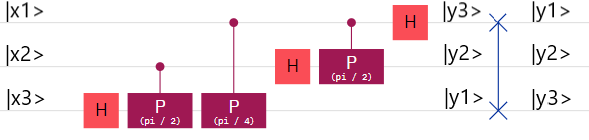
\includegraphics[width=\columnwidth]{qft.PNG}
\centering
\end{figure}

Anhand der Implementierung wird ersichtlich,
dass die Quanten-Fourier-Transformation unitär ist. 
Diese Eigenschaft ergibt sich aus der Tatsache, 
dass der zugehörige Quantenschaltkreis ausschließlich unter Verwendung von unitären Gattern realisierbar ist.

Wie bereits oben erwähnt, 
wird für die Rücktransformation aus der Fourierbasis in die Standardbasis 
die inversen Quanten-Fourier-Transformation angewendet.
Um einen Quantenschaltkreis aus unitären Gattern zu invertieren, 
wird die inverse der verwendeten Gatter
in umgekehrter Reihenfolge der originalen Schaltung angewendet.
Die Swap Operationen stehen somit bei der inversen Quanten-Fourier-Transformation am Anfang.
In Abbildung~\ref{fig:iqft} ist beispielhaft die inverse Quanten-Fourier-Transformation für drei Qubits abgebildet.
\begin{figure}
\caption{3-Qubit inverse QFT ohne Swaps}
\label{fig:iqft}
%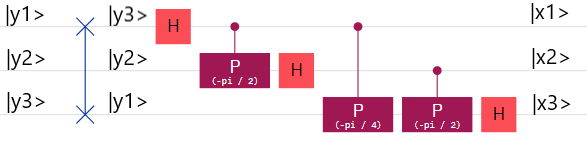
\includegraphics[width=\columnwidth]{iqft.PNG}
\centering
\end{figure}

\subsection{Quanten-Phase-Estimation} \label{Quanten-Phase-Estimation}

Im nachfolgenden Abschnitt wird die Anwendung und Funktionsweise des Quantum-Phase-Estimation Quantenalgorithmus erläutert. 
Die Quantum-Phase-Estimation ist ein Bestandteil einiger fortgeschrittener Quantenalgorithmen und eine integrale Komponente des spezifischen Quantenalgorithmus, 
der in dieser Arbeit implementiert wird. 
Genauer gesagt basiert der implementierte Algorithmus auf den Prinzipien der Quantum-Phase-Estimation und verwendet die selbe Methodik für einen spezialisierten Kontext.

Schwerpunktmäßig konzentriert sich die Erklärung primär auf das Verständnis der Funktionsweise der Quantum-Phase-Estimation und nimmt an, dass einige Voraussetzungen gegeben sind. 
Diese Voraussetzungen hängen vom spezifischen Kontext ab, 
in dem die Quantum-Phase-Estimation angewendet wird. 
Im weiteren Verlauf der Arbeit werden diese Voraussetzungen im Hinblick auf den Anwendungsfall des implementierten Quantenalgorithmus konkretisiert.

Voraussetzungen ist, dass ein Eigenvektor \(\ket{x}_n\) von einer unitäre Transformation \(U^{n\times n}\) bekannt ist.
Wendet man die Transformation \(U^{n\times n}\) auf \(\ket{x}_n\) an, 
so gilt: \(U^{n\times n}\ket{x}_n=\lambda_x\ket{x}_n\)~\cite{nielsen_chuang_2010}.
Dabei erhält man, abhängig vom gewählten Eigenvektor \(\ket{x}_n\), einen der Eigenwert \(\lambda_x\) von \(U^{n\times n}\).
Ein Eigenwert \(\lambda_x\) besitzt die Form eines Phasenfaktors: \(e^{2\pi i \varphi}\)
mit \(0 \leq \varphi < 1\).
Im Prinzip wird durch die unitäre Transformation also eine globale Phasenverschiebung auf den Eigenvektor angewendet.

Wie bereits im Kapitel zu den Grundlagen gezeigt wurde, 
ist es nicht möglich eine globale Phase durch eine gewöhnliche Messung der Qubits zu bestimmen. 
Das liegt daran, 
dass eine globale Phase die Amplituden eines Qubits nicht verändert und somit die Wahrscheinlichkeiten der Messergebnisse unverändert bleiben.
Stattdessen muss man die Qubits manipulieren, so dass die globale Phase doch Einfluss auf die Amplituden hat.

Der Quanten-Phase-Estimation Quantenalgorithmus ist in der Lage, 
den Eigenwert aus \(U^{n\times n}\ket{x}_n=\lambda_x\ket{x}_n\), also die Phasenverschiebungen, repräsentiert durch \(\lambda_x = e^{2\pi i \varphi}\),
auf die Amplitude eines anderen Qubits zu verschieben.
Um \(\lambda_x\) auf ein anderes Qubit zu übertragen wird der Effekt des \textbf{Phase-Kickback} genutzt.
Anschließend wird der Wert \(\varphi\) des Eigenwertes durch die inverse Quanten-Fourier-Transformation in einen messbaren Zustand überführt.

Der Phase-Kickback tritt auf,
wenn eine unitäre Transformation \(U^{n\times n}\) kontrolliert durch ein Qubit \(\ket{y}_1\) in Superposition, 
auf einen Eigenvektor \(\ket{x}_n\) von \(U^{n\times n}\) anwendet wirkt.
Dabei wird der Eigenwert, beziehungsweise \(\lambda_x\), auf den \(\ket{1}\)-Anteil von \(\ket{y}_1\)
übertragen.

Sei: \(\ket{y}_1 \equiv \alpha\ket{0} + \beta\ket{1}\) mit \(\alpha,\beta \neq 0\), 
dann:

\(CU^{(n+1)\times (n+1)}(\ket{y}_1\bigotimes\ket{x}_n)=(\alpha\ket{0} + \lambda_x\beta\ket{1})\bigotimes\ket{x}_n\).

Es folgt ein Beispiel welches den Effekt verdeutlicht:
Beachtet werden zwei Qubits im Zustand \(\ket{+}_1 \bigotimes \ket{-}_1\) auf die ein kontrolliertes X-Gatter angewendet wird.
Dabei ist \(\ket{-}_1\) der Eigenvektor einer X-Transformation mit zugehörigen Eigenwert \(-\), also \(X^{1\times 1}\ket{-}_1=-\ket{-}_1\).

Auf das zweite Qubit \(\ket{-}_1\) wirkt ein \(CX^{2\times 2}\) Gatter welches durch das erste Qubit \(\ket{+}_1\) kontrolliert wird:
\[
  CX^{2\times 2}( \ket{+}_1\ \bigotimes \ket{-}_1) =
  \begin{pmatrix}
    1 & 0 & 0 & 0\\
    0 & 1 & 0 & 0\\
    0 & 0 & 0 & 1\\
    0 & 0 & 1 & 0
  \end{pmatrix}
  \cdot
  \frac{1}{{2}}
  \begin{pmatrix}
    1 \\
    -1 \\
    1 \\
    -1 
  \end{pmatrix}
  =
  \frac{1}{{2}}
  \begin{pmatrix}
    1 \\
    -1 \\
    -1 \\
    1 
  \end{pmatrix}
  \]
  \[
  =
  \frac{1}{{\sqrt{2}}}
  \begin{pmatrix}
    1 \\
    -1 
  \end{pmatrix}
  \bigotimes
  \frac{1}{{\sqrt{2}}}
  \begin{pmatrix}
    1 \\
    -1 
  \end{pmatrix}
  =
  \ket{-}_1 \bigotimes \ket{-}_1
  \]
Mithilfe des Phase-Kickback kann man also den Eigenwert einer unitären Transformation in die Phase eines Kontrollqubits verschieben.
Der Vorteil davon ist, dass diese Phasenverschiebung nur den Vorfaktor von \(\ket{1}\) des Kontrollqubits betrifft und keine globale Phase darstellt.

Der Aufbau eines Quanten-Phase-Estimation Quantenschaltung sieht beispielsweise wie folgt aus:

Beachtet wird die unitäre Transformation eines Phase-Gatter(P) mit einer variablen Phasenverschiebung von 
\(P(2 i \pi \varphi ) = 
\begin{pmatrix}
  1 & 0\\
  0 & e^{2 i \pi \varphi}
\end{pmatrix}\).

Ein zugehöriger Eigenvektor dieser Transformation ist \(\ket{1}_1\) den \(P(2 i \pi \varphi)\ket{1}_1 = e^{2 i \pi \varphi} \ket{1}_1\).

Um den Effekt das Phase-Kickback nutzen zu können, muss sich das Kontrollqubit in einer Superposition befinden.
Dafür wird das Kontrollqubit im Zustand \(\ket{0}_1\) initialisiert und
anschließend mit einem Hadamard-Gatter(H) in die gleichmäßige Superposition \(\ket{+}_1\) versetzt.
\[\ket{0}_1 \bigotimes \ket{1}_1 
\underrightarrow{H^{\bigotimes 1}}
 \ket{+}_1 \bigotimes \ket{1}_1
=
\frac{1}{\sqrt{2}}
\begin{pmatrix}
  1 \\
  1
 \end{pmatrix}
 \bigotimes
 \begin{pmatrix}
  0 \\
  1 
 \end{pmatrix}
 =
 \frac{1}{\sqrt{2}}
 \begin{pmatrix}
  0 \\
  1 \\
  0 \\
  1
\end{pmatrix}
 \]
Über das kontrollierte Phase-Gatter wird der Eigenwert auf das Kontrollqubit verschoben und
befindet sich deswegen nicht mehr im Zustand \(\ket{+}_1\) :
\[
  \frac{1}{\sqrt{2}}
  \begin{pmatrix}
   0 \\
   1 \\
   0 \\
   1
  \end{pmatrix}
  \underrightarrow{CP^{2\times 2}(2 i \pi \varphi)}
  \begin{pmatrix}
    1 & 0 & 0 & 0\\
    0 & 1 & 0 & 0\\
    0 & 0 & 1 & 0\\
    0 & 0 & 0 & e^{2 i \pi \varphi}
  \end{pmatrix}
  \cdot
  \frac{1}{\sqrt{2}}
  \begin{pmatrix}
   0 \\
   1 \\
   0 \\
   1
  \end{pmatrix}
  =
  \frac{1}{\sqrt{2}}
  \begin{pmatrix}
    0 \\
    1 \\
    0 \\
    e^{2 i \pi \varphi}
  \end{pmatrix}
  =
  \frac{1}{\sqrt{2}}
  \begin{pmatrix}
    1 \\
    e^{2 i \pi \varphi}
   \end{pmatrix}
   \bigotimes
   \begin{pmatrix}
    0 \\
    1 
   \end{pmatrix}
  \]
Anschließend wird auf die Kontrollqubits die inverse Quanten-Fourier-Transformation angewendet.
Die inverse Quanten-Fourier-Transformation sorgt dafür, 
dass der Eigenwert die Amplituden der Kontrollqubits beeinflusst.
Die Qubits mit dem Eigenvektor sind für den weiteren Ablauf der Quanten-Phasen-Estimation nicht mehr relevant 
und werden nicht weiter beachtet.
Im Beispiel entspricht die inverse Quanten-Fourier-Transformation einem Hadamard-Gatter da nur ein einzelnes Kontrollqubit existiert:
\[
\frac{1}{\sqrt{2}}
\begin{pmatrix}
  1 \\
  e^{2 i \pi \varphi}
 \end{pmatrix}
 \underrightarrow{H^{\bigotimes 1}}
 \frac{1}{\sqrt{2}}
 \begin{pmatrix}
  1 & 1\\
  1 & -1
 \end{pmatrix}
 \cdot
 \frac{1}{\sqrt{2}}
\begin{pmatrix}
  1 \\
  e^{2 i \pi \varphi}
 \end{pmatrix}
 =
 \frac{1}{2}
 \begin{pmatrix}
  1 + e^{2 i \pi \varphi}\\
  1 - e^{2 i \pi \varphi}
 \end{pmatrix}
\]
Anhand des Ergebnisses des Beispiels ist zu erkennen, dass der Eigenwert praktisch auf die Amplitude vom Kontrollqubit transformiert wird.

Verwendet man ein Phase-Gatter mit \(\varphi  = 0.075\) sieht der Quantenschaltkreis wie in Abbildung~\ref{fig:qpe_1qubit} aus.
Mit dieser Phasenverschiebung sollte man bei einer Messung mit einer Wahrscheinlichkeit von ungefähr
\(0.9455\) den Zustand \(\ket{0}\) erhalten und \(\ket{1}\) mit der Wahrscheinlichkeit \(0.0544\).
Die Ergebnisse von 20.000 Messungen in Abbildung~\ref{fig:qpe_1qubit_Messung} bestätigen die Größenordnung der Wahrscheinlichkeiten.
Jedoch ergeben die Messungen aus Abbildung~\ref{fig:qpe_1qubit_Messung} nicht ganz genau den ausgerechneten Wahrscheinlichkeiten.
Dies liegt an der probabilistischen Natur der Messung.
Bei einer zunehmenden Anzahl an Messungen würden die Ergebnisse an die Wahrscheinlichkeitswerte konvergieren.
Somit benötigt man sehr viele Durchläufe des Quantenalgorithmus um anhand der Messungen ein verlässliches Ergebnis zu erhalten.

Es ist möglich die Präzision der Quanten-Phase-Estimation zu verbessern, 
indem mehr Qubits verwendet werden.
Diese Qubits werden dann als weitere Kontrollqubits verwendet.
Die Anzahl der Qubits für den Eigenvektor bleibt gleich der Bitanzahl, 
die ausreicht, um den Wert des Eigenvektors zu definieren.
Jedes einzelne Kontrollqubit kontrolliert ein \(U^{2^x}\)-Gatter.
Bei \(n\) Kontrollqubits kontrolliert das least-significant-bit ein \(U^{2^0}\)-Gatter,
das darauffolgende ein \(U^{2^1}\)-Gatter,
während das letzte Kontrollqubit ein \(U^{2^{n-1}}\)-Gatter kontrolliert.
Dabei kann \(U^{2^x}\) als \(2^x\) viele \(U\)-Gatter realisiert werden oder 
als ein einzelnes Gatter, welches den Eigenwert \(\lambda\) mit \(2^x\) multipliziert anwendet.
Anschließend wirkt die inverse Quanten-Fourier-Transformation auf alle Kontrollqubits.
Anhand der Messung kann dann \(\varphi\) bestimmt werden.
Der Aufbau der Schaltung ist in Abbildung~\ref{fig:qpe_n_qubit} abgebildet.

Wird die Quanten-Fourier-Transformation wie in Abbildung~\ref{fig:qpe_n_qubit} realisiert,
kann man den Zustand der Kontrollqubits vor der inversen Quanten-Fourier-Transformation wie folgt beschreiben:
\[\frac{1}{\sqrt{N}}[
  (\ket{0} + CU^{2^0}\ket{1}) \bigotimes
  (\ket{0} + CU^{2^1}\ket{1}) \bigotimes 
  ... \bigotimes
  (\ket{0} + CU^{2^{n-1}}\ket{1}) 
]\]
Mit \(U^{n\times n}\ket{x}_n=e^{2\pi i \varphi}\ket{x}_n\) wird der Eigenwert \(e^{2\pi i \varphi}\) wegen des Phase-Kickbacks
über die \(CU\)-Gatter auf die Kontrollqubits übertragen:
\[\frac{1}{\sqrt{N}}[
  (\ket{0} + e^{2\pi i 2^0 \varphi}\ket{1}) \bigotimes
  (\ket{0} + e^{2\pi i 2^1 \varphi}\ket{1}) \bigotimes 
  ... \bigotimes
  (\ket{0} + e^{2\pi i 2^{n-1} \varphi}\ket{1}) 
]\]
Schreibt man \(\varphi\) als Binärbruch:
\[\varphi = \frac{\varphi_n}{2^1} + \frac{\varphi_{n-1}}{2^2} + ... + \frac{\varphi_1}{2^n}\]
Kann die Formel in einer ähnlichen Form wie die Quanten-Fourier-Transformation umgeformt werden~\cite{nielsen_chuang_2010}:
\[\frac{1}{\sqrt{N}}[
  (\ket{0} + e^{2\pi i (\frac{\varphi_n}{2})} ... e^{2\pi i (\frac{\varphi_2}{2^{n-1}})}e^{2\pi i (\frac{\varphi_1}{2^{n}})}\ket{1})  ... 
  (\ket{0} +  e^{2\pi i (\frac{\varphi_2}{2})}e^{2\pi i (\frac{\varphi_1}{4})}\ket{1}) \bigotimes 
  (\ket{0} + e^{2\pi i (\frac{\varphi_1}{2})}\ket{1}) 
]\]
Die Formel besitzt die gespiegelte Struktur wie die Quanten-Fourier-Transformation ohne Swap-Gatter:
\[QFT_{N}\ket{x}_{n} = \frac{1}{\sqrt{N}}(\ket{0} + { e^{2 \pi i \frac{(x_1)}{2}}}\ket{1}) \bigotimes
( \ket{0} + { e^{2 \pi i \frac{(x_2)}{2}\frac{(x_1)}{4}}}\ket{1})...
(\ket{0} + e^{2\pi i (\frac{x_n}{2})} ... e^{2\pi i (\frac{x_2}{2^{n-1}})}e^{2\pi i (\frac{x_1}{2^{n}})}\ket{1})\]
Durch die Verwendung der Swap Gatter kann die Reihenfolge der quanten-Fourier-Transformation gespiegelt werden, 
anschließend sind beide Formeln strukturell identisch.

Wie im Kapitell zur Quanten-Fourier-Transformation erklärt,
transformiert die Quanten-Fourier-Transformation den Zustand der Eingangsqubits \(\ket{x}_n\) in die Phasen der Ausgangsqubits.
Hingegen kehrt die inverse Quanten-Fourier-Transformation diesen Vorgang um, 
indem die Phaseninformationen der Eingangsqubits in Zustände der Standartbasis transformiert werden.

Die Anwendung der inversen Quanten-Fourier-Transformation, inklusive Swap-Gatter, bewirkt also:
\[iQFT(\frac{1}{\sqrt{N}}[
  (\ket{0} + e^{2\pi i (\frac{\varphi_n}{2})} ... e^{2\pi i (\frac{\varphi_2}{2^{n-1}})}e^{2\pi i (\frac{\varphi_1}{2^{n}})}\ket{1})  ... 
  (\ket{0} +  e^{2\pi i (\frac{\varphi_2}{2})}e^{2\pi i (\frac{\varphi_1}{4})}\ket{1}) \bigotimes 
  (\ket{0} + e^{2\pi i (\frac{\varphi_1}{2})}\ket{1}) 
])\]
\[ = \ket{\varphi_1 \varphi_{2}...\varphi_n}_n = \ket{2^n\varphi}_n\]
Schließlich kann \(\varphi\) mit einer division durch \(2^n\) bestimmt werden.

Als Beispiel wird die Quanten-Phase-Estimation für
\(U^{1\times 1}\ket{1}_1=e^{2\pi i \frac{3}{8}}\ket{1}_1\) also mit \(\varphi = \frac{3}{8}\)
beachtet.
Damit der Quantenschaltkreis in Abbildung~\ref{fig:3_qubit_qpe} möglichst gut erkennbar ist,
werden die kontrollierten \(U^{2^x}\)-Gatter werden als Phase-Gatter mit \(P(e^{2^x 2\pi i \frac{3}{8}})\) realisiert.
\begin{figure}
  \caption{3-Kontroll-Qubit QPE}
  \label{fig:3_qubit_qpe}
  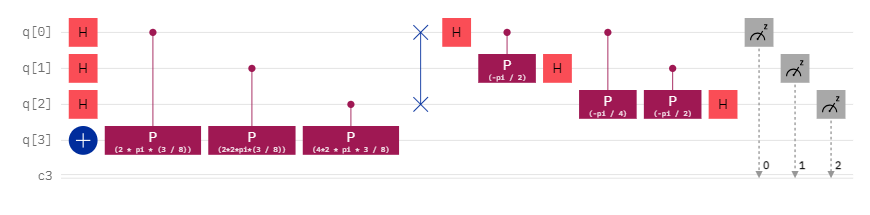
\includegraphics[width=\columnwidth]{3_qubit_qpe.png}
  \centering
  \end{figure}
Die Messung in Abbildung~\ref{fig:3_qubit_qpe_measurement} ergibt konsistent bei allen Durchläufen den Zustand \(\ket{3}_3\).
Da \(\ket{3}_3 = \ket{2^3\varphi}_3\) entspricht, kann mit einer Division \(\varphi = \frac{3}{8}\) bestimmt werden.
Es ist zu beachten, dass die Reihenfolge der Wertigkeit der Qubits gleich bleibt.
Normalerweise vertauscht die inverse wie auch die normale Quanten-Fourier-Transformation die Wertigkeiten.
Jedoch wird dieser Effekt mit Swap-Gattern korrigiert.
\begin{figure}
\caption{3-C-Qubit QPE Messergebnis}
\label{fig:3_qubit_qpe_measurement}
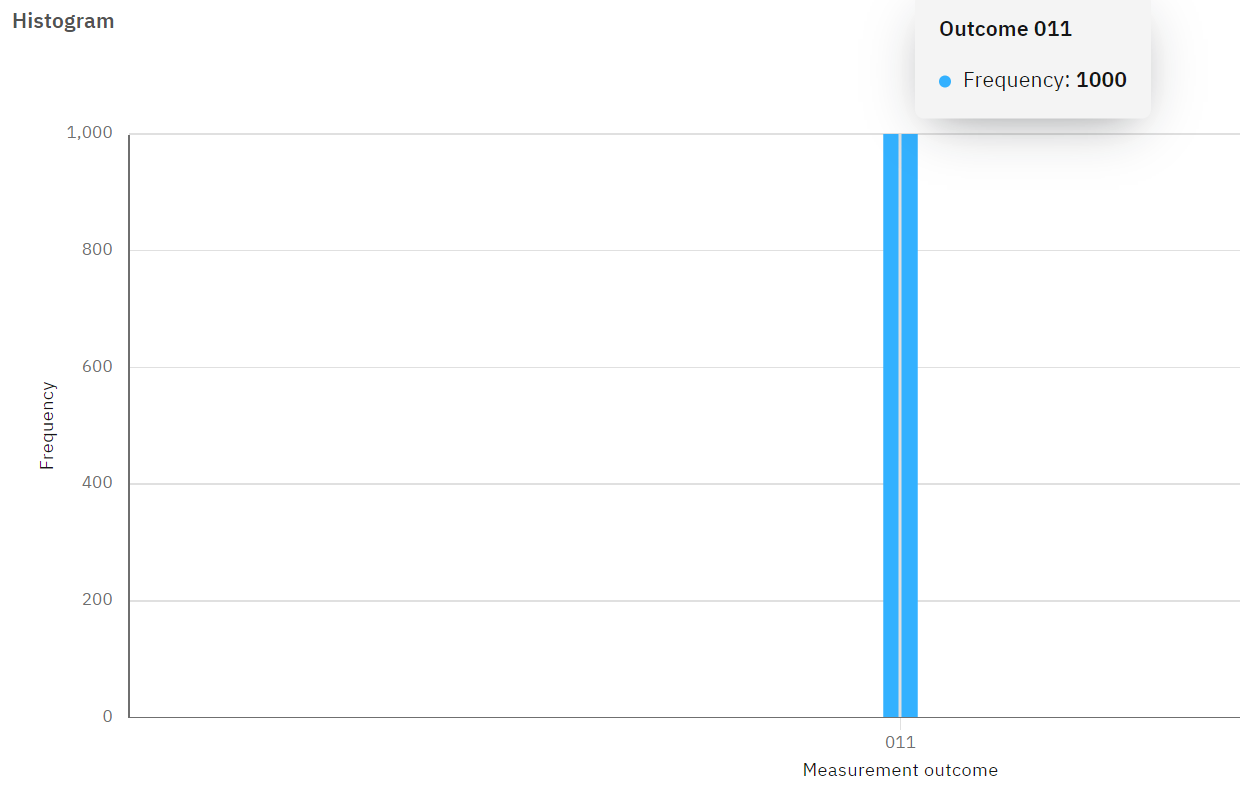
\includegraphics[width=\columnwidth]{3_qubit_qpe_measurement.PNG}
\centering
\end{figure}

Im vorherigen Beispiel liefern die Messungen aller Durchläufe den gleichen Zustand mit dem \(\varphi\) eindeutig bestimmbar ist.
Diese Eindeutigkeit tritt auf wenn die verwendete Anzahl an Kontroll-Qubits ausreicht, 
um \(\varphi\) eindeutig zu repräsentieren.
Im oberen Beispiel kann \(\varphi\) eindeutig mit den drei verwendeten Kontrollqubits dargestellt werden:
\({\frac{3}{8} =0 \cdot 2^{-1} + 1\cdot2^{-2} + 1\cdot2^{-3}}\).
Verwendet man nicht ausreichend Kontroll-Qubits kann \(\varphi\) nicht eindeutig repräsentiert werden.
Als Konsequenz wird die Messung ungenau.
Mit hoher Wahrscheinlichkeit kollabieren die Qubits bei einer Messung 
in die darstellbaren Zustände, die den genauen Wert am besten approximieren.
In Abbildung ~\ref*{fig:3_qubit_qpe_measurment_uncertain} sind die Messergebnisse von einer Quanten-Phase-Estimation
abgebildet, die die Phase \(\varphi = \frac{5}{16}\) bestimmen soll.
Da \(\frac{5}{16}\) nicht mit 3-Qubits darstellbar ist, gibt es kein eindeutiges Messergebnis.
Anhand der Messergebnisse ist aber erkennbar, dass die Messungen mit hoher Wahrscheinlichkeit,
zu den bestmöglichen Zuständen kollabieren.
Diese entsprechen \({\frac{2}{8} = \frac{4}{16}}\) und \({\frac{3}{8} = \frac{6}{16}}\), 
also genau die Werte um \(\frac{5}{16}\).


\begin{figure}
  \caption{QPE unpräzises Messergebnis}
  \label{fig:3_qubit_qpe_measurment_uncertain}
  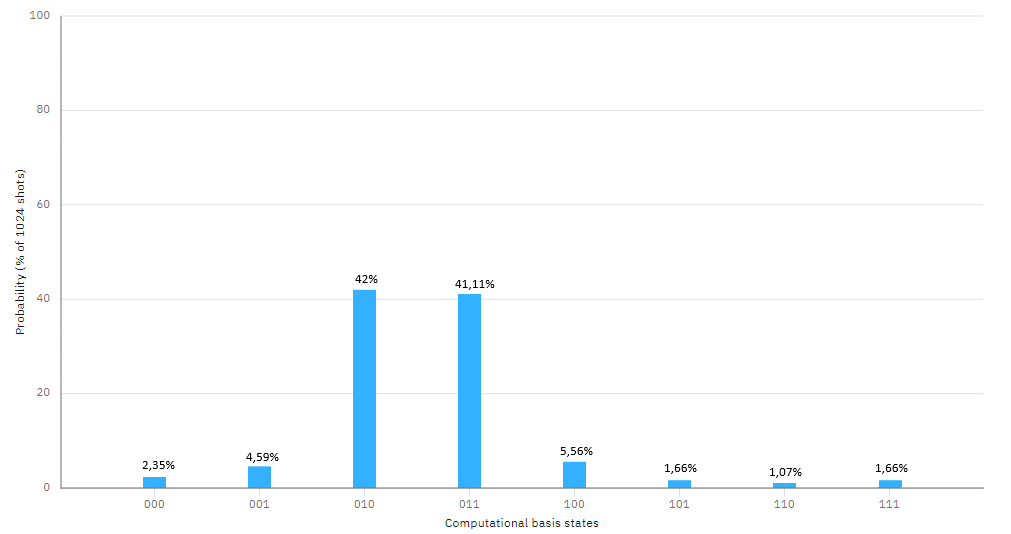
\includegraphics[width=\columnwidth]{3_qubit_qpe_measurment_uncertain.PNG}
  \centering
  \end{figure}












 






 











